\subsubsection{Business}

In figura \ref{model_business} è mostrato il modello di business. \\

L'Entità principale del modello è \texttt{Contract}, è una classe astratta che viene implementata da \texttt{Agreement} e \texttt{Funding}.
\texttt{Agreement}, che rappresenta una Convenzione, e \texttt{Funding} che rappresenta il Contributo differiscono fra loro solo per i campi dedicati all'Iva. La classe \texttt{Contract} possiede
tutti gli attributi comuni alle sue sottoclassi come \texttt{wholeTaxableAmount, approvalDate, deadlineDate}, etc.


\texttt{Contract} ha inoltre un insieme di \texttt{Installment}, un insieme di \texttt{Attachments}, un \texttt{ChiefScientist}
,un \texttt{Company} e infine una \texttt{ContractShareTable}

\texttt{ChiefScientist} rappresenta il Responsabile Scientifico, ogni convenzione/contributo ha un proprio responsabile.
\texttt{Company} rappresenta una ditta, la convenzione/contributo ha un riferimento alla dittà con cui ha stipulato l'accordo.
\texttt{Attachemnt} è la classe che rappresenta un allegato, la convenzione/contributo possiede un insieme di allegati.
\texttt{ContractShareTable} invece rappresenta la tabella di ripartizione di una convenzione/contributo: i suoi campi indicano come viene ripartito l'importo totale della convenzione/contributo fra il personale, l'ateno, etc.
La tabella di ripartizione ha inoltre un riferimento alla classe \texttt{StandardContractShareTabelFiller} implementazione concreta di \texttt{ContractShareTableFiller} che rappresenta una strategia per il riempimento della tabella in base
a normative definite.\texttt{Installment} è la classe che rappresenta le rate, una convenzione/contributo ha un insieme di rate; \texttt{Installment} ha due implementazioni concrete: \texttt{AgreementInstallment} e \texttt{FundingInstallment} rispettivamente
per convenzioni e contributi. \texttt{Installment} ha inoltre un riferimento a \texttt{InstallmentShareTable}. \texttt{InstallmentShareTable} e \texttt{ContractShareTable} estendono la stessa classe base \texttt{AbstractShareTable}.



\begin{figure}[h]
  \caption{Diagramma delle classi}
  \label{model_business}
  \centering
    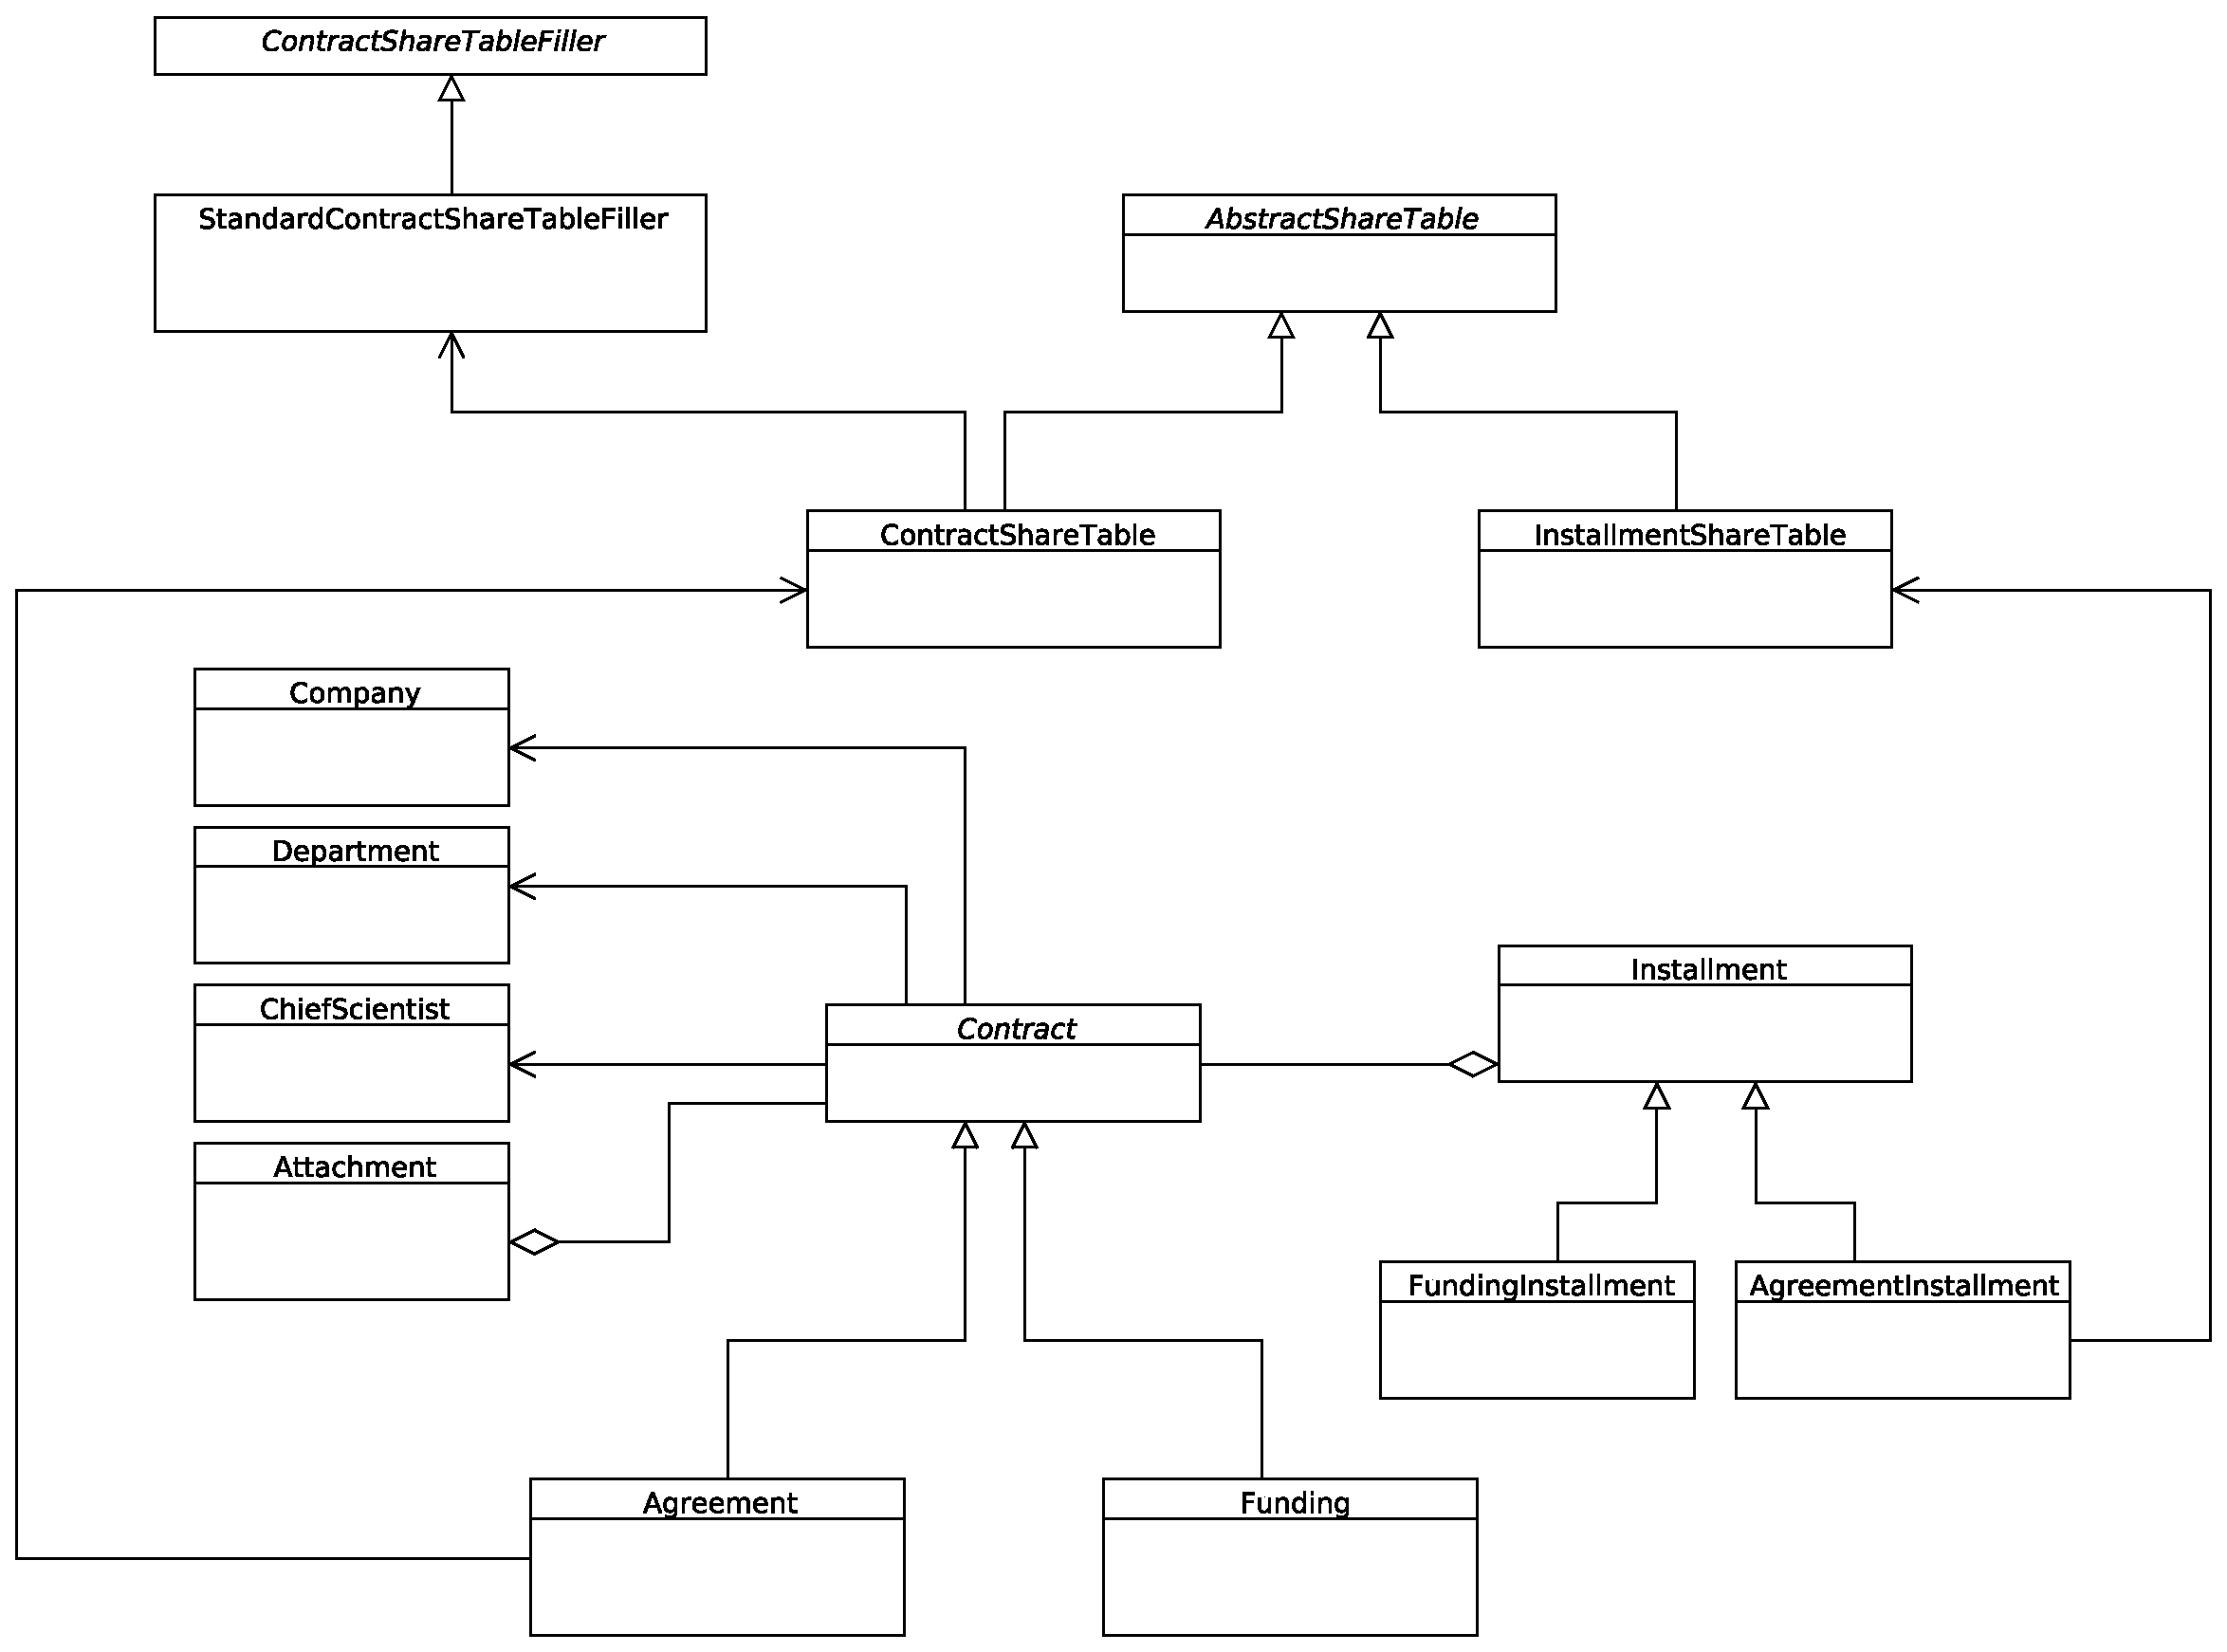
\includegraphics[width=1\textwidth]{images/modello_business.eps}
\end{figure}
